\chapter{ATAS Experiments in Germanium}

\section{Introduction}

\section{Experimental Considerations}

\subsection{sample requirements}

\begin{figure}
	\centering
	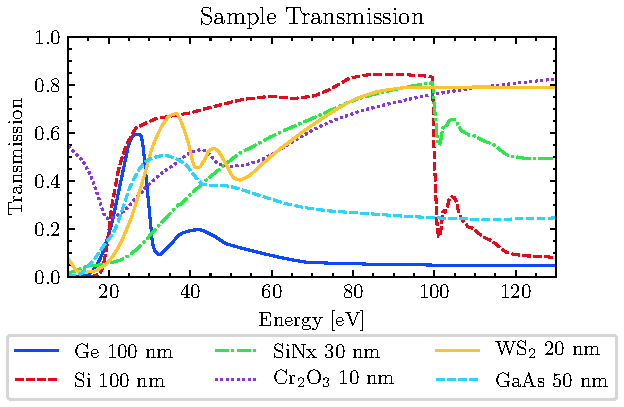
\includegraphics[width=0.75\textwidth]{figures/chap4/Sample_transmission_CXRO.pdf}
	\caption{Calculated XUV transmission of various materials. Data from \cite{gulliksonCXROXRayInteractions}.}
	\label{fig:Sample_trans_CXRO}
	% figure generated using \PythonScripts\CXRO\test\CXRO.py
\end{figure}

There are several sample requirements for a successful condensed matter transient absorption experiment. First and foremost, the sample needs to have an absorption edge within the bandwidth of the XUV source. Second, the material must be the correct thickness for a transmission measurement, given the capabilities of the XUV light source and detector. If the material is too thick, the ground state will absorb most of the XUV flux and the recorded spectrum will be too close to the noise floor of the apparatus. If it is too thin, the laser-induced change of the ground state (on the order of $1-10\%$) will be lost in the noise. As a general guideline, a sample that absorbs 50\% at the spectral feature of interest provides a good compromise between these conflicting requirements. \cref{fig:Sample_trans_CXRO} shows the expected transmission of several materials, calculated from the atomic scattering factors \cite{gulliksonCXROXRayInteractions}. We can see that a typical sample will be on the order of 10 - 200 nm thick, depending on the material.

Another upper bound for sample thickness comes from material dispersion. In any material, the XUV light ($n_{\text{IR}} \sim 1$) will outpace the IR light ($n_{\text{IR}} > 1$). This effect can be significant even for ultrathin films. In order to keep the phase slippage between the XUV and IR light below half an IR period, the sample thickness $L$ must obey the following relationship:
\begin{equation}
L \le \frac{1}{2} \frac{\lambda_{\text{IR}}}{n_{\text{IR}} - n_{\text{XUV}}}
\end{equation}
For germanium excited with $\lambda_{\text{IR}}$ = 1430 nm and probed with 30 eV XUV at the $M_{4,5}$ edge, $n_{\text{IR}}$ = 4.2481 \cite{nunleyOpticalConstantsGermanium2016} and $n_{\text{XUV}}$ = 0.992536 \cite{gulliksonCXROXRayInteractions}, which gives a maximum thickness of 220 nm.

Next, the sample needs to be excitable using laser sources present in our lab (i.e., ultrafast pulses with wavelengths between 800 nm and a couple of microns). To minimize the slow build up of heat (on the order of seconds) and laser-induced damage, the sample needs to be rastered through the laser focus as the experiment is performed. This rastering method necessitates both a large clear aperture ($\sim$ 1 mm$^2$ - 1 cm$^2$) and good sample uniformity. Samples that meet the above thickness and clear aperture requirements are extremely delicate, with thicknesses between 5,000 and 100,000 times smaller than their freestanding lateral dimensions. As such, one should expect most samples to break before, during and after measurements, so a successful experiment will have a materials pipeline that is capable of producing multiple, consistent samples in a short time frame.

\subsection{The Supporting Nitride Membrane}

\begin{figure}
	\centering
	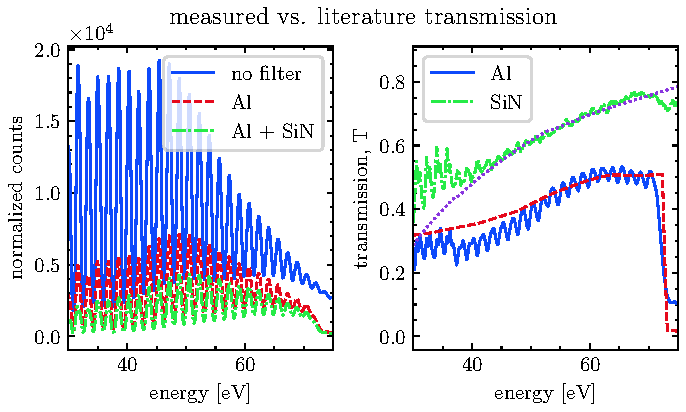
\includegraphics[width=0.75\textwidth]{figures/chap4/SiN_Al_transmission.pdf}
	\caption{XUV transmission measurements of Al metallic filter and silicon nitride membrane. Left panel: normalized XUV counts for i) unfiltered HHG signal, ii) HHG going through a 200 nm Al filter and iii) HHG going through a 200 nm Al filter and 30 nm of silicon nitride. Counts are scaled by the Jacobian. Right panel: transmission curves obtained from the left panel's data. Also shown are literature values for 20 nm of silicon nitride and 200 nm of Al with two 4 nm oxide layers \cite{gulliksonCXROXRayInteractions}. Multilayer interference is not taken into account. Oscillations in measured transmission are numerical artifacts which will be discussed in the text.}
	\label{fig:SiN_Al_transmission}
	% dataset: \2019_05_02\
	% plotted using: \Python Scripts\Spectrometer\test\nitride_trans.py
\end{figure}

\begin{figure}
	\centering
	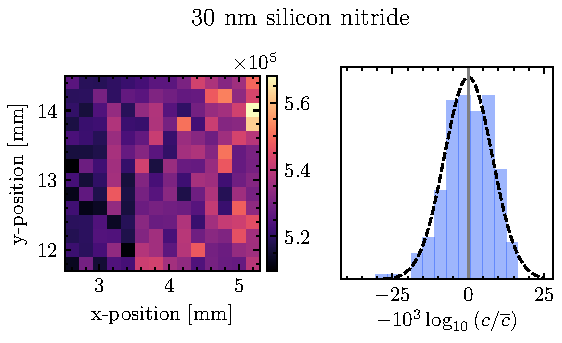
\includegraphics[width=0.75\textwidth]{figures/chap4/nitride_map.pdf}
	\caption{XUV transmission map of 30 nm silicone nitride freestanding membrane. Left panel: integrated XUV counts in the range 30 -- 34 eV. Sample holder motor positions are indicated by x- and y-positions. Right panel: histrogram of logarithmic deviation of counts from the average. Dashed line shows a normal distribution.}
	\label{fig:nitride_map}
	% figure created using \Python Scripts\Spectrometer\test\rastermap.py
	% dataset: C:\testdata\2019_09_10\4_55_32 PM_nitride_map1
\end{figure}

\begin{figure}
	\centering
	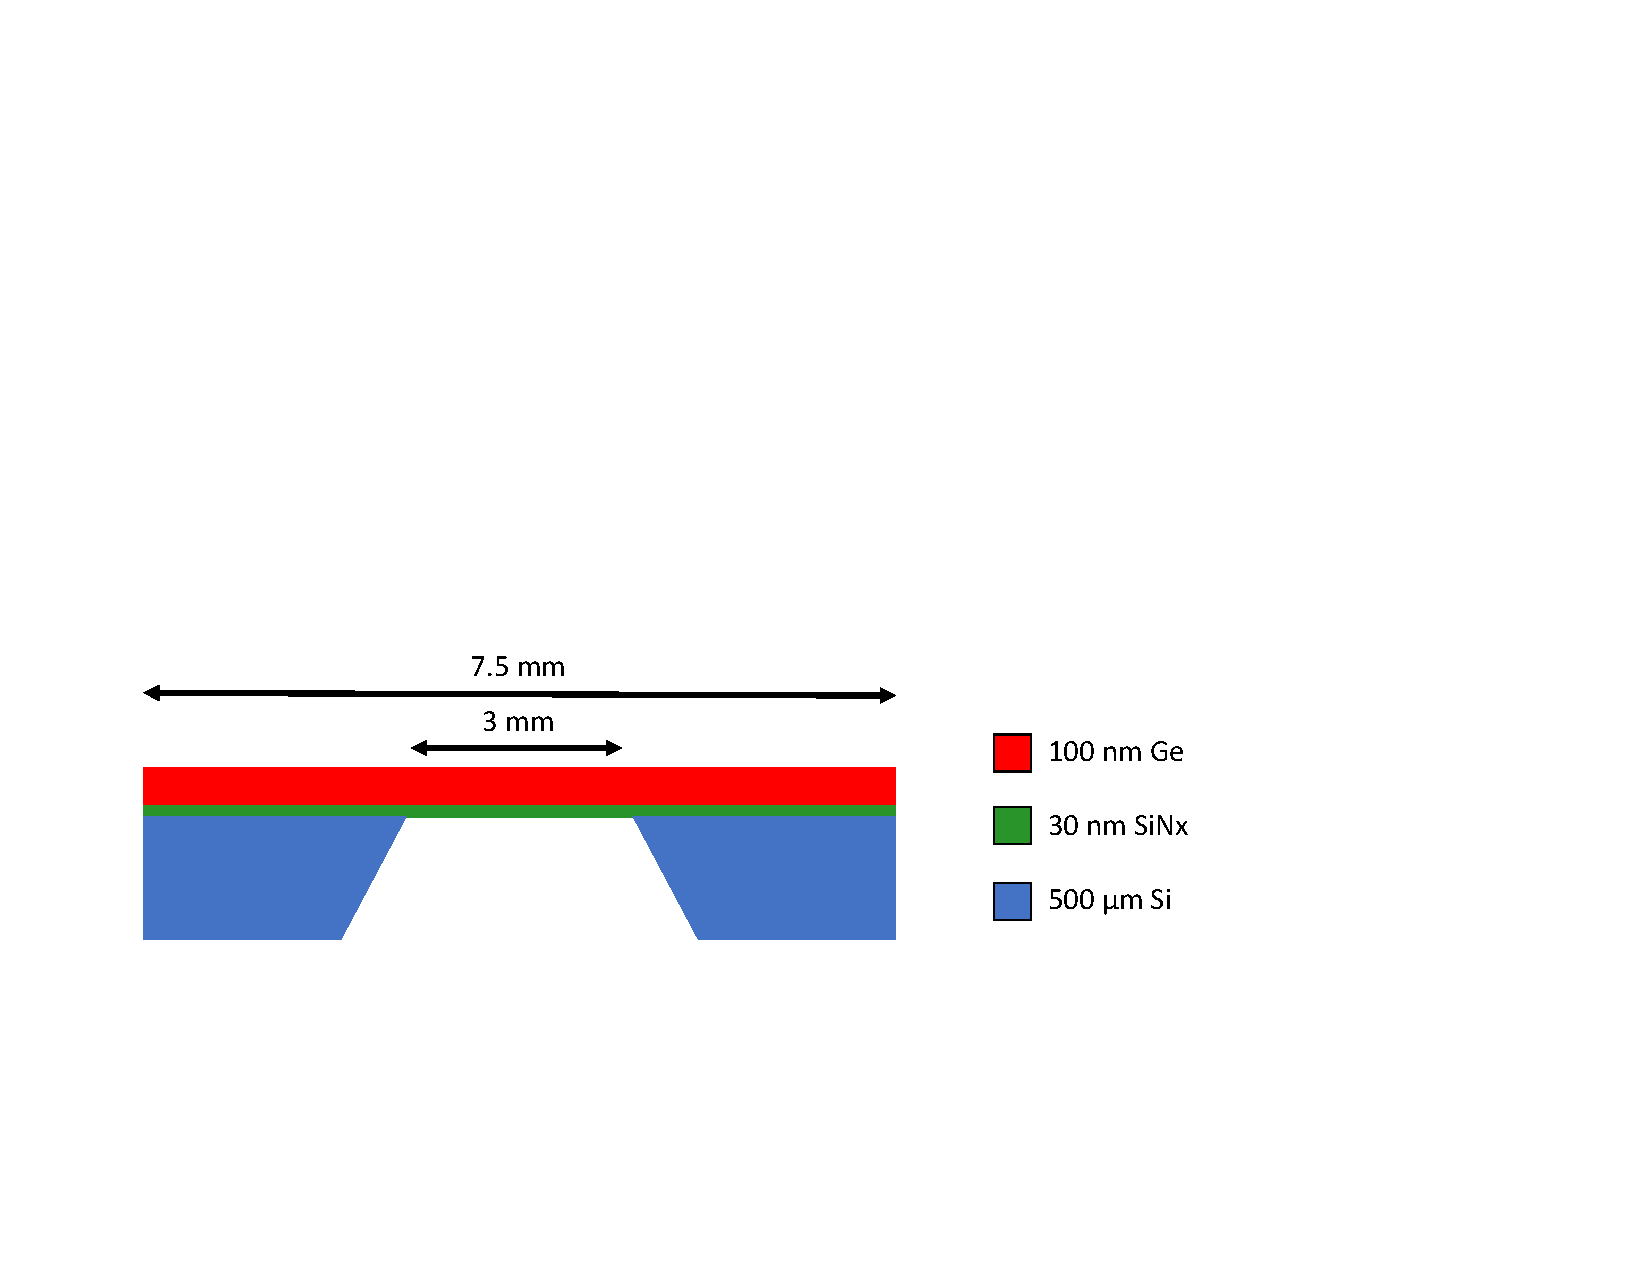
\includegraphics[width=0.75\textwidth]{figures/chap4/Sample_Geometry.pdf}
	\caption{Cartoon showing the cross section of the free standing sample heterostructure. A 500 $\mu$m thick Si frame supports a freestanding 30 nm low stress silicon nitride membrane (Norcada QX7300X), upon which 100 nm of germanium has been deposited. The Si frame has a 3x3 mm$^2$ square clear aperture and a 7.5x7.5 mm$^2$ square external dimension. The taper of the Si frame thickness along the perimeter of the clear aperture forms a knife edge. In an ATAS experiment, the XUV and IR pulses propagate from the top to bottom of the figure.}
	\label{fig:Sample_Geometry}
\end{figure}

While most materials have an absorption edge within the range 25 - 150 eV, there are very few commercially available pre-fabricated materials with both the requistite large clear aperture and thickness. Note that either characteristic is relatively easy to achieve individually, but their combination presents unique materials challenges. We considered three synthesis methods to produce this quasi-2D sample:
\begin{enumerate}
	\item sample growth on a traditional substrate, followed by chemical back-etching or milling of the substrate until sub-micron thickness of the heterostructure is achieved;
	\item sample growth on a traditional substrate, followed by mechanical transfer onto a membrane;
	\item sample growth on a membrane.
\end{enumerate}
Sample quality and composition is heavily impacted by local growth conditions such as substrate temperature, deposition rate, substrate crystal cut, substrate-sample lattice mismatch, etc. Many of these characteristics are changed when growing on a substrate of a different cut, or by replacing a substrate with a membrane. In general, one should not expect success when applying a substrate-optimized growth recipe to a freestanding membrane. Therefore, methods 1 and 2 will yield the highest quality samples, as they leverage already-developed sample recipes. However, both methods require a technically difficult second step that is prone to failure.

Selective chemical etching recipes exist for certain compounds, but they usually require an additional chemically intert layer in the heterostructure to protect the sample. Adding this layer will come at the expense of the total XUV flux transmitted by the heterostructure. Additionally, the chemical etching rates are highly dependent on local chemistry, fluid convection and temperature \cite{chiuPhotoluminescenceEvolutionGaAs2015}, which ultimately means that the amount of material removed is uncontrollable and unrepeatable within our requirements (499.9 $\mu$m $\pm$ 10 nm removed from a 500 $\mu$m substrate). For these reasons, we decided to not pursue a chemical etch recipe. Ion or electron milling is more controllable, but too expensive to implement on a large scale. The above reasons preclude the use of Method 1.

Mechanical transfer of thin samples is a tried and true method, but it usually results in flakes with lateral dimensions on the order of 100 $\mu$m. Repeated transfer of many flakes is possible, but there little control over their exact positioning on the membrane. This results in a random distribution of flakes; the flakes are sometimes folded or overlapping one another. These mishaps increase the effective optical density of the sample, changing the IR and XUV absorption properties significantly.

An XUV spatial measurement needs to be taken prior to any ATAS experiment, but a non-uniform distribution of flakes on a membrane would require a much higher resolution map. This is because the flakes are on the order of the XUV and IR focii, so it is critical that the raster points in \cref{fig:Rastering_Methods} correspond to the center of each flake to avoid edge diffraction and to minimize the effects of slow laser pointing drift. For a uniform film, a map can be taken using 200-250 $\mu$m step sizes, as the most important feature is the border of the clear aperture. On the other hand, each flake would have to be sampled $\sim$5 times in each direction to find its center. As a conservative estimate, a membrane covered with $100 \times 100\text{ }\mu$m$^2$ flakes would require a step size of 20 $\mu$m, which increases the number of raster points by a factor of $10^2 = 100$. Considering that a $3 \times 3 \text{ mm}^2$ clear aperture sampled with 200 $\mu$m steps takes $\sim$45 minutes to map, a random distribution of flakes would take a prohibitively long time to map out.

With the first two methods ruled out, we turn to the third method of growing directly on a freestanding membrane. Although it will result in a lower quality sample, it does not have the same technical hurdles of the previous two methods. However, the large clear area makes the heterostructure extremely fragile. We initially attempted to circumvent this problem by using an array of smaller clear apertures.

As shown in \cref{fig:Rastering_Methods}, most of the sample's area isn't directly used by the laser - it exists as a buffer between the grid of sample points. An alternative to a single clear aperture is an array of micro-apertures, each with a diameter on the order of the IR spot size. The micro-apertures exist within a mechanically robust substrate and a thin membrane lies on top of the structure. This configuration significantly eases the material strength requirements by reducing the size of the unsupported area from cm-scale to sub-mm-scale. The regular grid of apertures avoids the difficulties of a randomly distributed sample, easing the XUV mapping step size requirements. Fortunately, these arrays are commercially available from Silson, Norcada (silicon nitride membranes) and US Applied Diamond (diamond membranes) but we encountered technical difficulties in their implementation. Because the aperture size is on the order of the size of the IR focal spot, there is very little room for positioning error, and our motors were insufficiently precise for this application. Further, these arrays are typically only available in at most a $3\times3$ array, which provides an insufficient number of raster points for an ATAS experiment.

With these limitations in mind, we decided to use large aperture x-ray windows from Norcada. These windows consist of a mechanically robust Si frame substrate with a square clear aperture cut through the center. The structure is fabricated so that a thin membrane covers the clear aperture. A schematic of the cross section is shown in \cref{fig:Sample_Geometry}.

Norcada offers these structures with either a silicon (polycrystalline or single-crystal) or a silicon nitride membrane. An ideal membrane is transparent to both XUV and IR wavelengths with a high damage threshold. Referring to \cref{fig:Sample_trans_CXRO}, 100 nm of Si provides a relatively flat transmission curve from 25 to 100 eV. In constrast, 30 nm of silicon nitride has poor, but featureless, transmission at lower energies. Both materials transmit light below their bandgaps (5 eV for SiN and 1.14 eV for Si). Finally, silicon nitride's higher bandgap results in a significantly higher laser damage threshold \cite{gamalyAblationSolidsFemtosecond2002,austinFemtosecondLaserDamage2018,keldyshIonizationFieldStrong1965}. Taking all these factors into account, we decided to use 30 nm silicon nitride membranes for germanium transient absorption experiments. The measured transmission of a typical membrane is shown in \cref{fig:SiN_Al_transmission}.


\subsection{rastering of sample through focus to avoid heating, charge build-up}

\begin{figure}
	\centering
	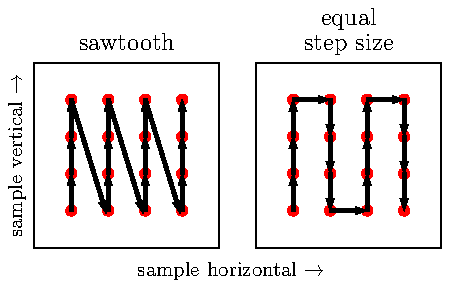
\includegraphics[width=0.75\textwidth]{figures/chap4/rastering_methods.pdf}
	\caption{Schematic of competing raster methods, shown in the sample's reference frame. The clear aperture of the sample is represented by the interior of the black square. The laser propagation direction is out of the page. The laser focal spots are shown as red circles, and the movement of the sample holder relative to the laser focus is indicated by arrows. A 200 $\mu$m border exists between the raster array and the perimeter of the sample's clear aperture. This diagram is to scale for a $1\times1$ mm$^2$ clear aperture sample, a 60 $\mu$m diameter IR focal spot and a 200 $\mu$m step size.}
	\label{fig:Rastering_Methods}
	%figure created using \Python Scripts\rastering\raster_diagram.py
\end{figure}

\subsection{XUV maps of samples}

\subsection{IR propagation in thin films (TMM starting with LightPipes output)}

\begin{figure}
	\centering
	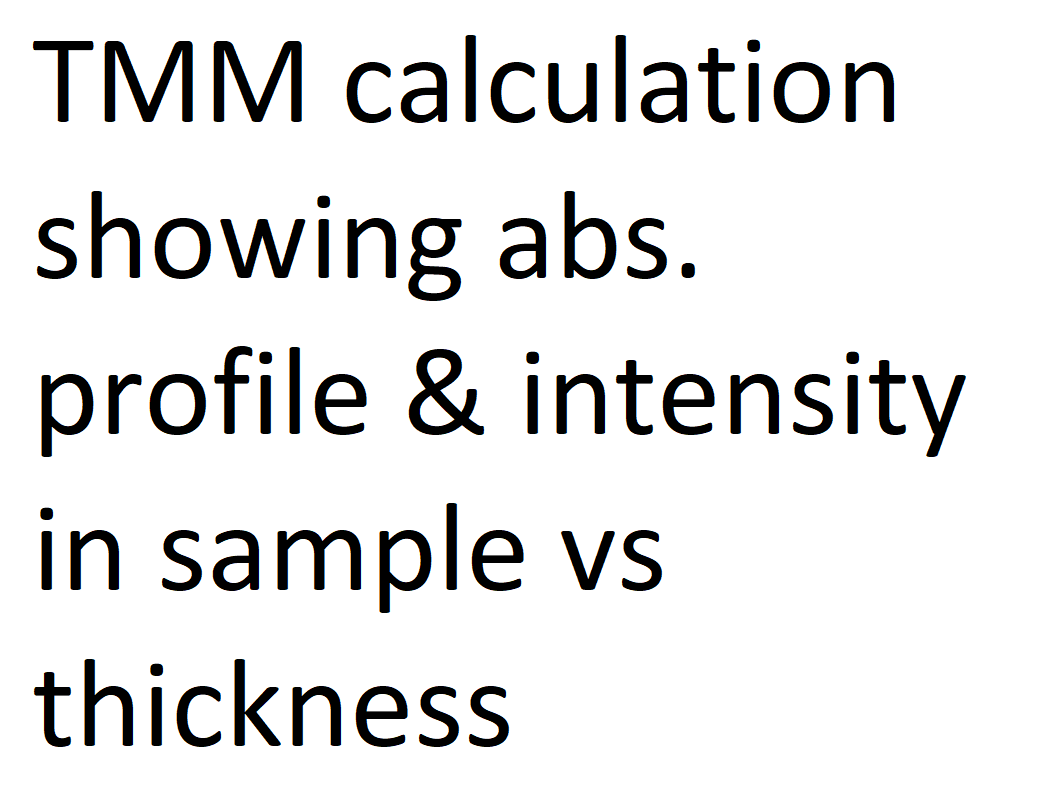
\includegraphics[width=0.75\textwidth]{figures/chap4/TMM_calc.png}
	\caption{thin film calculation made using the TMM package \cite{byrnesTmmSimulateLight2017,byrnesMultilayerOpticalCalculations2019}.}
	\label{fig:thin_film_calc}
\end{figure}


\subsection{orbital-resolved excitation probability vs wavelength (band structure calculations)}

\begin{figure}
	\centering
	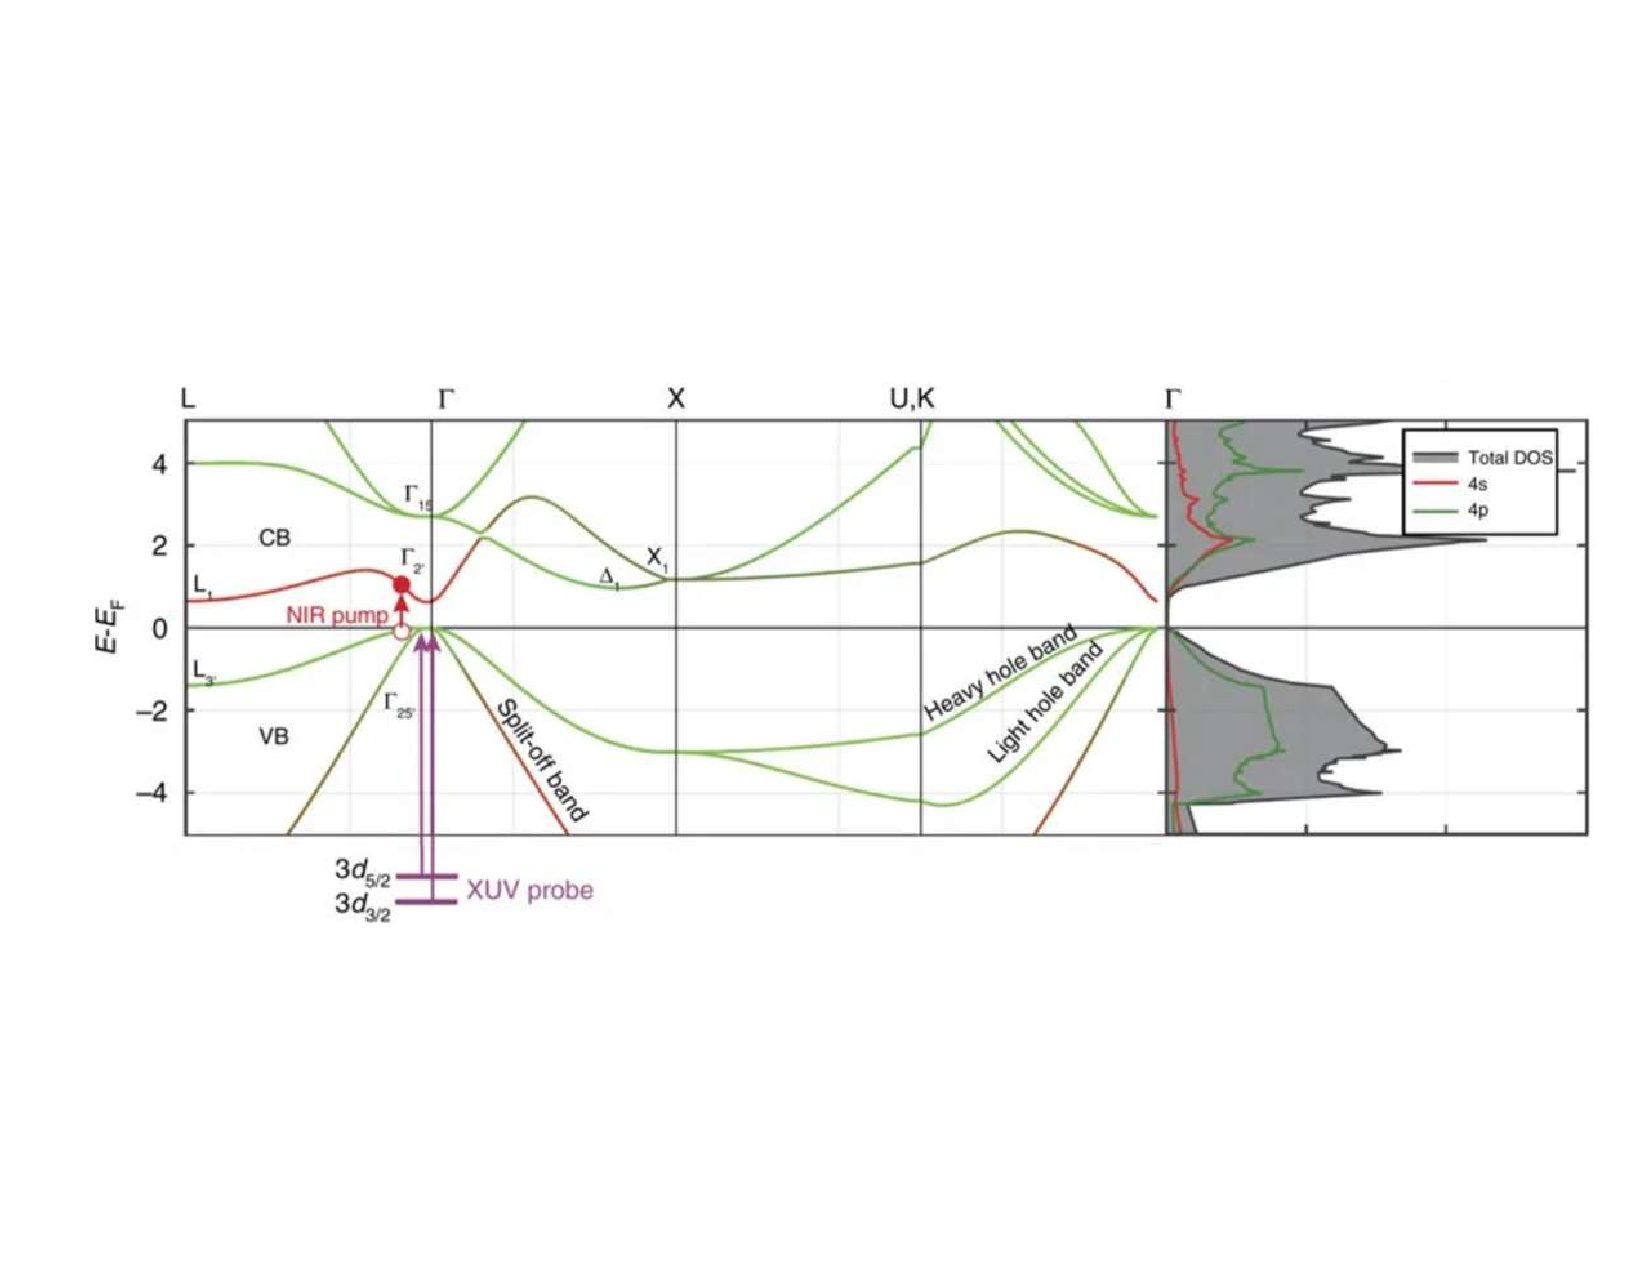
\includegraphics[width=0.75\textwidth]{figures/chap4/Ge_band_diagram_Zurch2017.pdf}
	\caption{Band structure and orbital character of germanium. Purple arrows indicate XUV-induced transitions from the $3d$ core levels to the valence bands. Red arrow indicates IR-induced transition across the direct band gap. Figure adapted from \cite{zurchDirectSimultaneousObservation2017}.}
	\label{fig:Ge_band_diagram}
\end{figure}


\subsection{laser damage}

\subsection{estimation of excited carrier density}

\textbf{need to include orbital-resolved excitation probability results in this section}

We are concerned with two quantities: the peak excitation fraction in the sample and the average excitation fraction at the location of the XUV focus. The former quantity is relevant when considering sample damage, whereas the latter will be proportional to the measured signal. If the XUV and IR spots are perfectly overlapped at the sample plane, then these two quantities are approximately equal. We first calculate the peak excitation fraction, then we consider how a misaligned beam will affect the measured signal.

The laser propagation calculations in \cref{fig:pump_on_focus_calculation} were done for vacuum, but we are concerned with the field in our sample. The electric field inside a dielectric $E_{\text{int}}$ is related to the external electric field by the following equation \cite{schultzeAttosecondBandgapDynamics2014}:
\begin{equation}
E_{\text{int}} = \frac{2}{1+\sqrt{\epsilon}} E_{\text{ext}}
\label{eqn:internal_external_Efield}
\end{equation}
where $E_{\text{int}}$ is the electric field inside the sample, $E_{\text{ext}}$ is the electric field outside the sample, $\epsilon$ is the dielectric constant and its square root is the refractive index $n_{\text{IR}}$. The internal intensity $I_{\text{int}}$ is the square of the internal electric field. For germanium at $\lambda$ = 1430 nm, $n_{\text{IR}}$ = 4.2481, and we have the following relations:
\begin{equation}
\begin{aligned}
E_{\text{int}} &= 0.381 \times E_{\text{ext}} \\
I_{\text{int}} &= 0.145 \times I_{\text{ext}}
\end{aligned}
\end{equation}

Given our laser paremeters, we can estimate the highest carrier density within the sample. First, we estimate the absorbed laser fluence, $F_{\text{abs}}$ \cite{harbCarrierRelaxationLattice2006}:
\begin{equation}
F_{\text{abs}} = F_{\text{inc}} \left(1-R\right) \left( 1-\exp(-\alpha L) \right) \left(1+R \exp(-\alpha L)\right),
\label{eqn:absorbed_fluence}
\end{equation}
where $F_{\text{inc}}$ is the incident fluence, $R$ is the reflectivity equal to the square of the Fresnel coefficient, $\alpha$ is the absorption coefficient and $L$ is the sample thickness. The bracketed terms in \cref{eqn:absorbed_fluence} are the fraction of fluence transmitted by the first surface, the fraction absorbed by a single pass through the sample, and the additional absorption due to a back reflection off the rear face of the sample. Note that the back-propagating beam will arrive (on average) at a delay of $n_{\text{IR}} L/(2c) \approx 0.7 \text{ fs}$ later than the forward-propagating beam. This time scale is nearly two order of magnitude less than the IR pulse duration, so we should expect any electron dynamics initiated by the back reflection to contribute to the measured signal.

If each absorbed photon corresponds to an excited electron, then the excited carrier density $\Delta N$ is given by the following expression \cite{cushingDifferentiatingPhotoexcitedCarrier2019}:
\begin{equation}
\Delta N = \frac{F_{\text{abs}}}{\hbar \omega} \frac{1}{L},
\label{eqn:excitation_fraction}
\end{equation}
where $\hbar \omega$ is the IR photon energy. In \cref{eqn:excitation_fraction}, the quantity $F_{\text{abs}} / (\hbar \omega)$ represents the number of absorbed photons per unit area; dividing this quantity by the sample thickness gives the number of absorbed photons per unit volume. This assumes that the skin depth of the material is greater than membrane thickness, which is true for germanium at these wavelengths.

Finally, we convert the excited carrier density to a fractional excitation. Germanium has $N_{\text{u.c.}}=2$ valence electrons per unit cell, and each unit cell has a volume $V_{\text{u.c.}}=4.527 \times 10^{-23} \text{ cm}^{3}$. Therefore the fractional carrier excitation is
\begin{equation}
f = \Delta N \frac{V_{\text{u.c.}}}{N_{\text{u.c.}}}
\end{equation}

We can use literature values for 100 nm of germanium pumped at $\lambda$ = 1430 nm light. From the literature \cite{nunleyOpticalConstantsGermanium2016}, $R = 0.38315$, $\alpha = 5803.4 \text{ cm}^{-1}$, and so $F_{\text{abs}} = 0.0413 \times F_{\text{inc}}$. Therefore, only about 4.13\% of the incident fluence is absorbed by the sample.

According to the calculations in \cref{fig:pump_on_focus_calculation}, for each 1 $\mu$J energy input pulse (measured at L4), 0.413 $\mu$J makes it to the focal plane. 49\% of that energy is within the main lobe, which contains 0.202 $\mu$J of energy. Approximating the central lobe as a Gaussian beam with a FWHM of 35 $\mu$m and a pulse energy of 0.202 $\mu$J, the peak fluence is calculated by dividing the total energy of the Gaussian by $\pi w^2/2$. The Gaussian beam waist $w$ is related to the FWHM via $w^2 = \text{FWHM}^2 / (2 \ln 2)$. Thus, for each 1 $\mu$J input energy, the peak fluence in the central lobe is 14.6 mJ/cm$^2$ and the absorbed peak fluence is 0.60 mJ/cm$^2$. This corresponds to an peak excited carrier density of $4.3 \times 10^{20} \text{ cm}^{-3}$ and an excitation fraction of 0.98\% (per 1 $\mu$J of input energy).


\subsection{XUV-IR spatial overlap}

\begin{figure}
	\centering
	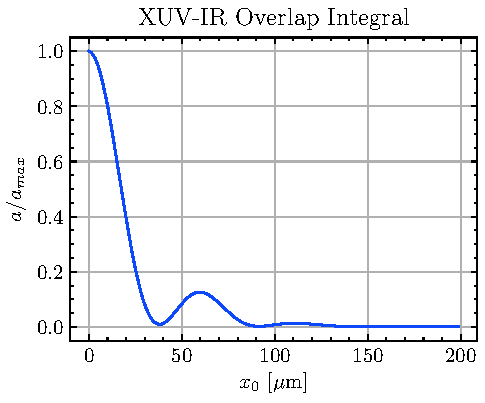
\includegraphics[width=0.5\textwidth]{figures/chap4/XUV-IR_overlap_integral.pdf}
	\caption{XUV-IR overlap function, as defined in \cref{eqn:XUV-IR_integral}, calculated using the numerical simulation results of \cref{fig:pump_on_focus_calculation} and a Gaussian XUV beam with a 6 $\mu$m waist. The result has been normalized to perfect overlap, $a_{max}$.}
	\label{fig:XUV-IR_integral}
	% plot made with \Python Scripts\LightPipes\pump_intensity.py using N=2**13 gridside
\end{figure}

The excitation fraction can be computed for each spatial coordinate on the sample using the above method and the predicted intensity distribution from the numerical beam propagation calculations. Because the electrons are being excited via a single-photon process, the excited carrier density will be proportional to the fluence, and thus proportional to the intensity shown in \cref{fig:pump_on_focus_calculation}. Because the intensity of the XUV is very weak, the absorption of the XUV by the sample is also linear. Thus, we should expect the ATAS signal to be proportional to the XUV-IR overlap integral:
\begin{equation}
a = \frac{ \int dV \text{ } I_{\text{IR}} I_{\text{XUV}} }{ \int dV \text{ } I_{\text{IR}} \int dV \text{ } I_{\text{XUV}} }
\label{eqn:XUV-IR_integral_volume}
\end{equation}
Here, the integration volume is over the entire sample. If we assume that the intensity distribution does not appreciably change over the thickness of the sample, we can simplify the above equation. This is a reasonable assumption because the sample ($L = 100 \text{ nm}$) is much thinner the Rayleigh range ($z_R \sim 1 \text{ mm}$), and the absorption is low ($\sim 4\%$). So we assume the sample is a $\delta$-function in thickness and only evaluate the intensities at the focal plane. With this assumption, the overlap integral becomes:
\begin{equation}
a = L \frac{ \int dA \text{ } I_{\text{IR}} I_{\text{XUV}} }{ \int dA \text{ } I_{\text{IR}} \int dA \text{ } I_{\text{XUV}} }
\label{eqn:XUV-IR_integral}
\end{equation}
Knife edge measurements have been performed on the XUV light, showing that it has a Gaussian spatial profile with a beam waist of 6 $\mu$m. We write down the spatial profile of the XUV light at the focus:
\begin{equation}
I^{XUV} = I_0^{XUV} \exp \left( - 2 ((x-x_0)^2 + (y-y_0)^2) /  w_{XUV}^2 \right)
\end{equation}
Here, $I_0^{XUV}$ is the peak intensity and $w_{XUV}$ is the beam waist (radius), defined as the point where the intensity falls to $e^{-2} = 13.5\%$ of its maximum. The lateral shift from the center of the IR focal spot in the horizontal and vertical directions is $x_0$ and $y_0$, respectively. With this formulation, and using the simulation results for the IR spot, the XUV-IR overlap integral is calculated as a function of XUV-IR misalignment $(x_0, y_0)$. This result is shown in \cref{fig:XUV-IR_integral}. Here, XUV beam is translated relative to the IR beam in the horizontal direction ($x_0$ with $y_0=0$) and the overlap is computed from \cref{eqn:XUV-IR_integral}.

\cref{fig:XUV-IR_integral} shows the sensitivity of a condensed matter ATAS experiment to relative alignment.\footnote{Note that the relevant parameter in \cref{eqn:XUV-IR_integral} is the relative positions of the two focal spots. We have yet to calculate the sensitivity of spatial overlap to deviations in the input laser pointing.} A spatial overlap deviation of 10 $\mu$m will cause the XUV-IR overlap - and thus the measured signal - to drop by 20\%. Note that a 10 $\mu$m displacement of the IR at the sample corresponds to a 15 $\mu$rad tilting of the hole mirror (HM). There are two ways misalignment can affect experimental results. If the relative positions of the XUV and IR focal spots changes as an experiment is performed, then the recorded ATAS signal would be a function of both the laser-induced dynamics and the XUV-IR spatial misalignment. On the other hand, if the entire experiment is performed using a constant misalignment, we would be exciting the sample to some peak excitation fraction $f$, but our probe would be measuring a lower excitation fraction ($\approx f a / a_{max}$). Consequently, the measured ATAS signal would be lower than otherwise expected, and any attempts to boost the signal by increasing the interaction intensity could result in permanent laser-induced sample damage.

A condensed matter ATAS experiment has much tighter alignment tolerances than a gas phase experiment. This discrepancy is a simple consequence of sample geometry and density. In either experiment, the measured signal comes from the region of space where the sample density, XUV intensity and IR intensity overlap. The transmission of XUV through the sample is, to first order, $T= \exp(- n \mu_a d)$, where $n$ is the number density, $d$ is the sample thickness and $\mu_a$ is the photoabsorption cross section. As discussed above, for technical reasons the experiment should be designed with $T \approx 1/2$. Therefore, the product $n \mu_a d$ will be approximately constant for any transient absorption experiment.

The number density of a condensed phase sample is determined by the chemistry of the compound and is on the order of $4 \times 10^{22} \text{ atoms}/\text{cm}^3$. The experimentalist is free to engineer clever sample geometries, heterostructures and/or nanopatterns, but the high atomic density (and thus absorption coefficient) dictates a total sample thickness on the order of 100 nm. On the other hand, the spatial profile and density of a gas phase sample is determined by the gas nozzle design and its backing pressure, respectively. A typical nozzle used in our lab produces a gas plume with lateral dimensions on the order of 200 - 500 $\mu$m. This effectively creates a sample that is three orders of magnitude thicker than a condensed phase sample, which relaxes the alignment constraints significantly. This has important consequences for the alignment of the sample.

If the XUV and IR are perfectly collinear, then the beam overlap region is effectively infinite in the propagation direction. In this case, the XUV-IR overlap integral will be positive regardless of any displacement of the sample plane from the focal plane, and maximal when the sample lies in the focal plane. However, if there is a small angle $\delta \theta$ between their $k$-vectors, then the beams will only spatially overlap within a finite region. In this case, the position of the sample plane relative to the beam crossing plane becomes a critical experimental parameter. For an infinitely thick sample (i.e., a chamber effusively filled with gas), it wouldn't matter where the beams crossed as long as they overlapped somewhere within the chamber. Then, the overlap integral would decrease as a function of $\delta \theta$, but it would never go to zero. For a thin sample, the bounds of \cref{eqn:XUV-IR_integral_volume} must enclose the beam overlap region, or else the integral will be zero. Thus, the signal strength of a condensed phase ATAS experiment is roughly 3 orders of magnitude more sensitive to the $z$-position of the sample relative to the focal plane than a gas phase ATAS experiment.


\section{Optimizing experimental ATAS parameters for Germanium thin films}

\subsection{rep rate (avoiding ms-scale excitation)}

\begin{figure}
	\centering
	\subfloat[$\tau \approx 0$ fs, PE = $1.03 \text{ } \mu \text{J}$.]{
		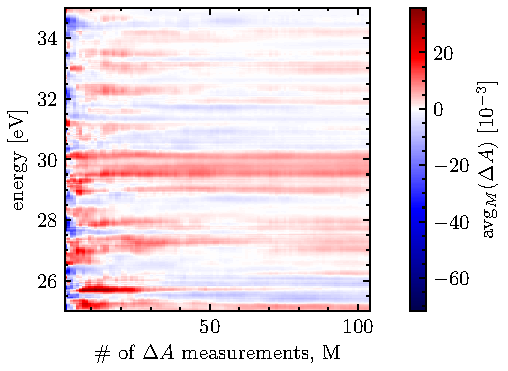
\includegraphics[width=0.4\textwidth]{figures/chap4/StaticOD_1kHz_overlap_1p03uJ.pdf}
		\label{fig:1kHz_Ge_ATAS:overlap_1.03uJ}}
	\qquad
	\subfloat[$\tau \approx 0$ fs, PE = $1.43 \text{ } \mu \text{J}$.]{
		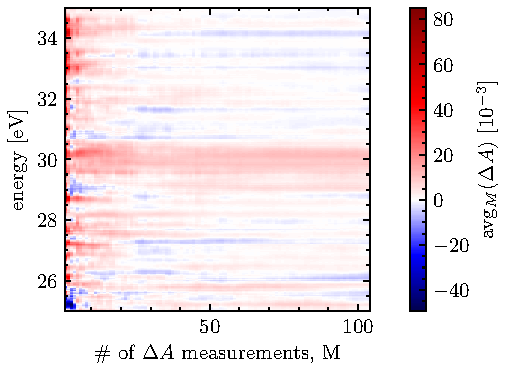
\includegraphics[width=0.4\textwidth]{figures/chap4/StaticOD_1kHz_overlap_1p43uJ.pdf}
		\label{fig:1kHz_Ge_ATAS:overlap_1.43uJ}}
	
	\subfloat[$\tau = - \infty$, PE = $1.03 \text{ } \mu \text{J}$.]{
		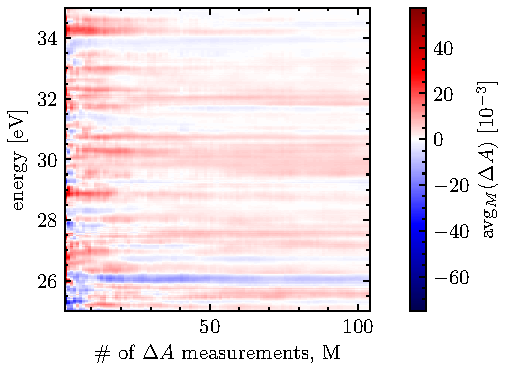
\includegraphics[width=0.4\textwidth]{figures/chap4/StaticOD_1kHz_NegInf_1p03uJ.pdf}
		\label{fig:1kHz_Ge_ATAS:NegInf_1.03uJ}}
	\qquad
	\subfloat[$\tau = - \infty$, PE = $1.43 \text{ } \mu \text{J}$.]{
		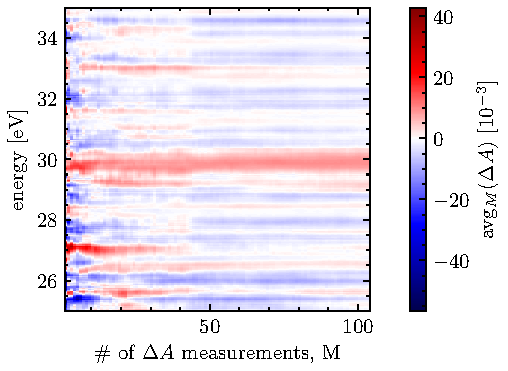
\includegraphics[width=0.4\textwidth]{figures/chap4/StaticOD_1kHz_NegInf_1p43uJ.pdf}
		\label{fig:1kHz_Ge_ATAS:NegInf_1.43uJ}}
	
	\subfloat[PE = $1.03 \text{ } \mu \text{J}$.]{
		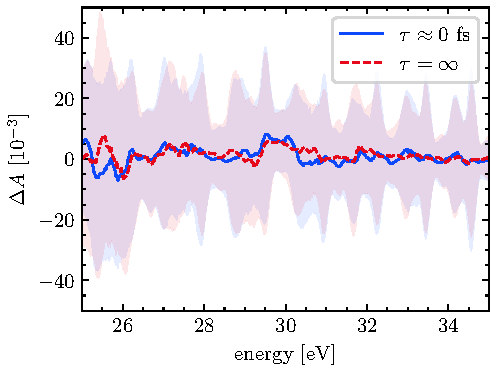
\includegraphics[width=0.4\textwidth]{figures/chap4/StaticOD_avg_1kHz_1p03uJ.pdf}
		\label{fig:1kHz_Ge_ATAS:avg_1.03uJ}}
	\qquad
	\subfloat[PE = $1.43 \text{ } \mu \text{J}$.]{
		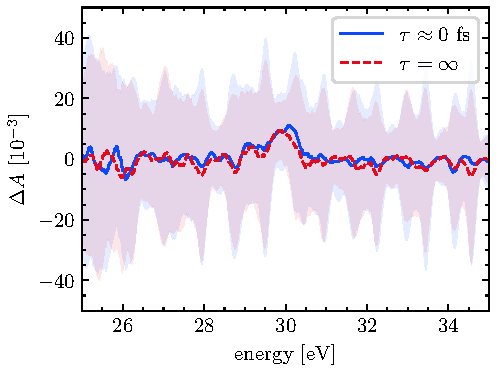
\includegraphics[width=0.4\textwidth]{figures/chap4/StaticOD_avg_1kHz_1p43uJ.pdf}
		\label{fig:1kHz_Ge_ATAS:avg_1.43uJ}}
	\caption{1 kHz fixed-delay ATAS measurements on 100 nm Ge using a $\lambda = 1450 \text{ nm}$ excitation pulse. See text for details.}
	\label{fig:1kHz_Ge_ATAS}
	% datasets: \testdata\2019_08_06\{Avg1,Avg3,Avg4,Avg5}
	% python script: \Python Scripts\Spectrometer\test\2019_08_06.py
\end{figure}

\begin{figure}
	\centering
	\subfloat[$\tau \approx 0$ fs, PE = $1.75 \text{ } \mu \text{J}$.]{
		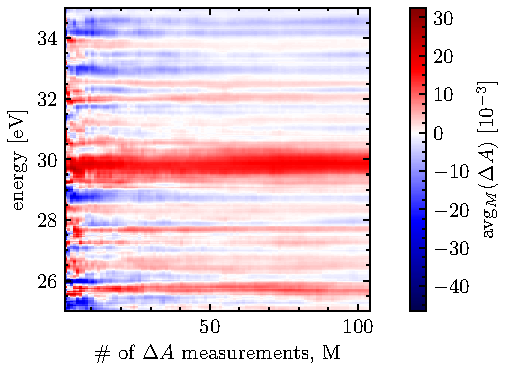
\includegraphics[width=0.4\textwidth]{figures/chap4/StaticOD_1kHz_overlap_1p75uJ.pdf}
		\label{fig:1kHz_Ge_ATAS:overlap_1.75uJ}}
	\qquad
	\subfloat[PE scaling at $\tau \approx 0$ fs.]{
		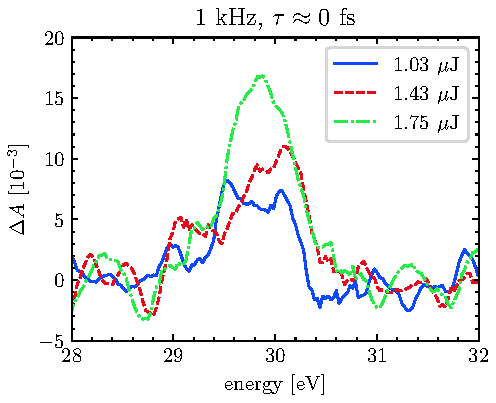
\includegraphics[width=0.4\textwidth]{figures/chap4/StaticOD_avg_1kHz_PE_scaling.pdf}
		\label{fig:1kHz_Ge_ATAS:PE_scaling}}
	
	\subfloat[PE = $1.43 \text{ } \mu \text{J}$.]{
		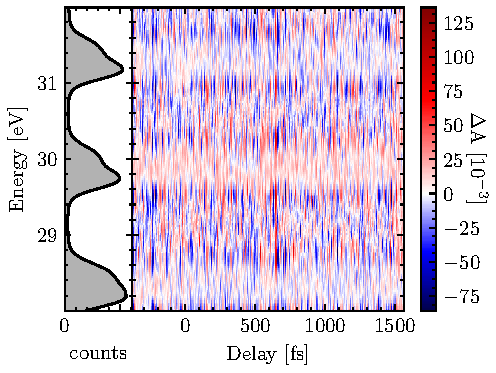
\includegraphics[width=0.4\textwidth]{figures/chap4/ODvsDelay_1kHz_1p43uJ.pdf}
		\label{fig:1kHz_Ge_ATAS:delay_1.43uJ}}
	\qquad
	\subfloat[PE = $1.75 \text{ } \mu \text{J}$.]{
		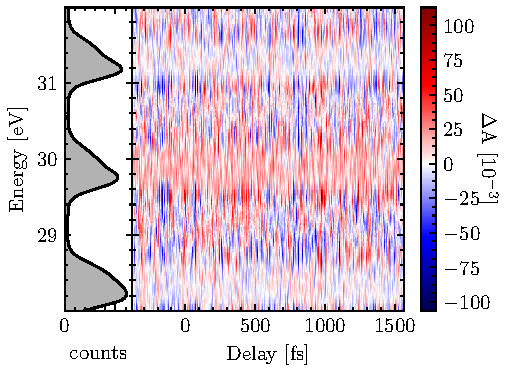
\includegraphics[width=0.4\textwidth]{figures/chap4/ODvsDelay_1kHz_1p75uJ.pdf}
		\label{fig:1kHz_Ge_ATAS:delay_1.75uJ}}
	
	\subfloat[PE = $1.43 \text{ } \mu \text{J}$ (rolling average).]{
		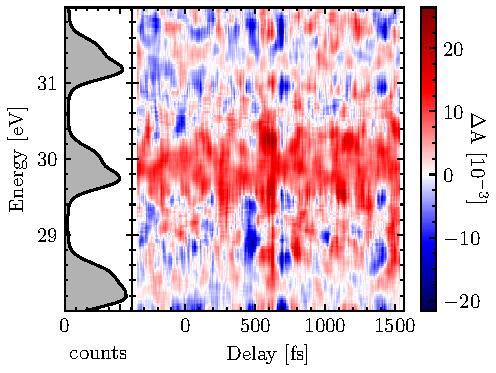
\includegraphics[width=0.4\textwidth]{figures/chap4/ODvsDelay_20roll_1kHz_1p43uJ.pdf}
		\label{fig:1kHz_Ge_ATAS:roll_delay_1.43uJ}}
	\qquad
	\subfloat[PE = $1.75 \text{ } \mu \text{J}$ (rolling average).]{
		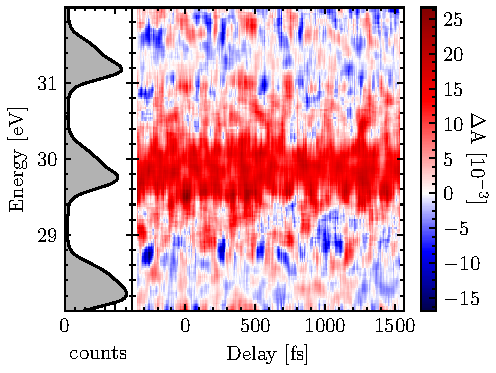
\includegraphics[width=0.4\textwidth]{figures/chap4/ODvsDelay_20roll_1kHz_1p75uJ.pdf}
		\label{fig:1kHz_Ge_ATAS:roll_delay_1.75uJ}}
	\caption{1 kHz ATAS measurements in Ge using a $\lambda = 1450 \text{ nm}$ excitation pulse. \cref{fig:1kHz_Ge_ATAS:overlap_1.75uJ}: fixed-delay ATAS measurements with a pulse energy of 1.75 $\mu$J. \cref{fig:1kHz_Ge_ATAS:PE_scaling}: Pulse energy scaling at overlap of 1 kHz measurements. \cref{fig:1kHz_Ge_ATAS:delay_1.43uJ,fig:1kHz_Ge_ATAS:delay_1.75uJ,fig:1kHz_Ge_ATAS:roll_delay_1.43uJ,fig:1kHz_Ge_ATAS:roll_delay_1.75uJ}: delay scans at 1 kHz.  \cref{fig:1kHz_Ge_ATAS:delay_1.43uJ,fig:1kHz_Ge_ATAS:delay_1.75uJ}: raw delay scan data. \cref{fig:1kHz_Ge_ATAS:roll_delay_1.43uJ,fig:1kHz_Ge_ATAS:roll_delay_1.75uJ}: rolling average of the raw data with a 65 fs window (20 delay points). The left panel on each spectrogram shows the ground state spectrum $S_{gs}(E)$. See text for details.}
	\label{fig:1kHz_Ge_ATAS:delay}
	% datasets: \testdata\2019_08_06\{Delay1,Delay2}
	% python script: \Python Scripts\Spectrometer\test\2019_08_06.py
\end{figure}

\begin{figure}
	\centering
	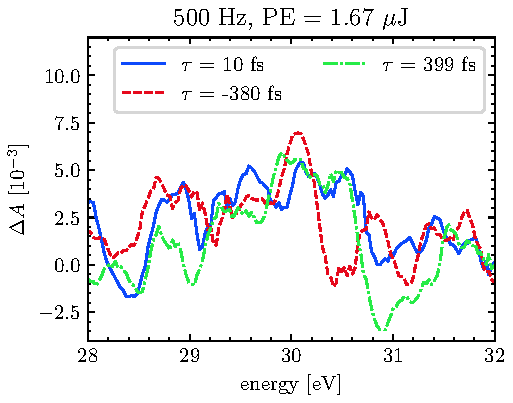
\includegraphics[width=0.75\textwidth]{figures/chap4/StaticOD_avg_500Hz_1p67uJ.pdf}
	\caption{500 Hz ATAS measurements in Ge using a $\lambda = 1450$ nm, 1.67 $\mu$J excitation pulse. Each delay curve is an average of 104 identical measurements. The sample shows no delay dependance within the uncertainty of the measurement.}
	\label{fig:500Hz_Ge_ATAS:delays}
	% dataset: C:\testdata\2019_08_06\HWP1{Avg8,Avg9,Avg10}
	% python file: \Python Scripts\Spectrometer\test\2019_08_06.py
\end{figure}

\begin{figure}
	\centering
	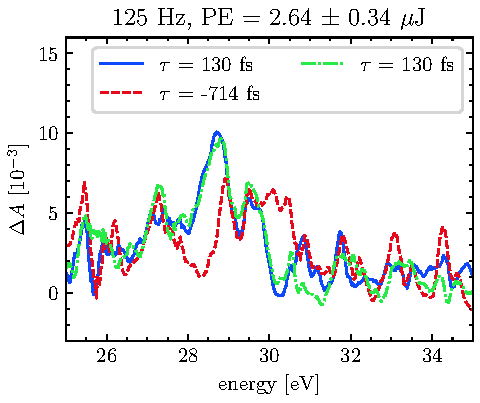
\includegraphics[width=0.75\textwidth]{figures/chap4/StaticOD_avg_125Hz_2p64uJ.pdf}
	\caption{125 Hz ATAS measurements in Ge using a $\lambda = 1450$ nm, 2.64 $\mu$J excitation pulse. Each lineout represents the average of 394 measurements. See text for details.}
	\label{fig:125Hz_Ge_ATAS:static_delays}
	% dataset: C:\testdata\2019_08_13\Avg1,2,3
	% python file: Python Scripts\Spectrometer\test\2019_08_13.py
\end{figure}

\begin{figure}
	\centering
	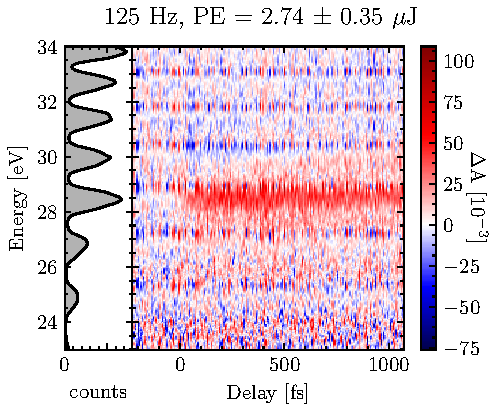
\includegraphics[width=0.75\textwidth]{figures/chap4/Delay234_1450nm_125HzuJ.pdf}
	\caption{125 Hz delay scan in Ge using a $\lambda = 1450$ nm, 2.74 $\pm$ 0.35 $\mu$J excitation pulse. This is an average of 3 repeated measurements. See text for details.}
	\label{fig:125Hz_Ge_ATAS:delay_scan}
	% dataset: C:\testdata\2019_08_13\Delay2,3,4 averaged together.
	% python file: Python Scripts\Spectrometer\test\2019_08_13.py
\end{figure}

We performed exploratory experiments at 1 kHz to determine the optimal excitation pulse energy. For this set of measurements, we generated harmonics in Argon using $\lambda$ = 1450 nm, a 200 nm Al filter and the $2C$ optics removed (see \cref{fig:beamline_schematic}). Two delay points were recorded: with the XUV and IR pulses overlapped ($\tau = 0$) and with the XUV pulse arriving about 300 fs before the IR ($\tau = -\infty$). For each delay point, we used three pulse energies: 1.03, 1.43 and 1.75 $\mu$J. To increase the signal-to-noise, we performed each experiment 104 times and averaged the datasets. The exposure time was 0.5 seconds, and the sample was rastered so that each measurement was recorded at a new position on the sample. The results are shown \cref{fig:1kHz_Ge_ATAS,fig:1kHz_Ge_ATAS:overlap_1.75uJ,fig:1kHz_Ge_ATAS:PE_scaling}. 

\cref{fig:1kHz_Ge_ATAS:overlap_1.03uJ,fig:1kHz_Ge_ATAS:overlap_1.43uJ,fig:1kHz_Ge_ATAS:NegInf_1.03uJ,fig:1kHz_Ge_ATAS:NegInf_1.43uJ,fig:1kHz_Ge_ATAS:overlap_1.75uJ} show the average $\Delta A$ as a function of the number of averaged measurements, $M$. Spectral features are apparent after averaging about 10 datasets together, but the fidelity of the signal does not appreciably improve after the first $M=50$ datasets. \cref{fig:1kHz_Ge_ATAS:avg_1.03uJ,fig:1kHz_Ge_ATAS:avg_1.43uJ} show the average signal (lines) and the standard deviation (shaded area), as calculated from the entire ensemble of measurements. The data is noisy, but we can see a spectral feature near 30 eV which scales with pulse energy (or perhaps average power). This behavior is evident in \cref{fig:1kHz_Ge_ATAS:PE_scaling}. However, this feature is delay-independent: $\Delta A$ has nearly the same value regardless of whether the XUV arrives before or after the IR pulse.

To confirm the delay-independence of this feature, we performed delay scans at two different pulse energies (1.43 and 1.75 $\mu$J). These measurements are shown in \cref{fig:1kHz_Ge_ATAS:delay}. Delay was controlled by inserting a fused silica wedge into the inteferometer (W in \cref{fig:beamline_schematic}). Each delay step corresponds to approximately 3.25 fs (25 $\mu$m of wedge insertion).

The raw data is shown in \cref{fig:1kHz_Ge_ATAS:delay_1.43uJ,fig:1kHz_Ge_ATAS:delay_1.75uJ}. As this experiment was only performed once ($M=1$), the contrast is poor and the 30 eV feature is barely visible. The spectral feature becomes more prominent after performing a rolling average over 20 delay points (65 fs), which is shown in \cref{fig:1kHz_Ge_ATAS:roll_delay_1.43uJ,fig:1kHz_Ge_ATAS:roll_delay_1.75uJ}. These delay measurements confirm our suspiscion that the absorption feature is delay-independent at 1 kHz.

One possible origin of a delay-independent signal can be a very long-lived excited state with lifetime $1/\Gamma$. Each laser shot initiates an assortment of electron and phonon dynamics, each with their own time scales. If any of these excited states have time scales that approach the inverse rep. rate of the laser ($1/RR$), then the dynamics from the previous shot will still be evolving by time the next shot arrives. Since each exposure integrates over hundreds or thousands of laser shots, measurements at a nomimal delay $\tau$ will contain information from several delays $\tau_i$, each separated by the time between laser shots: $\tau_i = \tau, \tau-\frac{1}{RR}, \tau-\frac{2}{RR}, \dots$, with the amplitude of each contribution weighed by an exponential decay factor $\exp(+ \tau_i \Gamma)$. If this is the case, then the magnitude of the delay-independent signal should decrease as time between laser shots is increased. As the time between laser shots is increased past the lifetime of the state, the excited state population from the previous laser shot will be small enough to observe the dynamics of the shorter-lived states. Experimentally, we can accomplish this by adjusting the rep. rate divider on the Spitfire amplifier (which reduces the rep. rate), and/or using an optical chopper.

The rep. rate was halved to 500 Hz using the Spitfire's rep. rate divider ($m=2$) and the exposure time was doubled to 1 second so that the number of laser shots per exposure was held constant. A series of fixed-delay measurements were recorded using a 1.67 $\mu$J pulse energy, shown in \cref{fig:500Hz_Ge_ATAS:delays}. The spectral feature at 30 eV is still present, but it does not exhibit any delay dependence within the uncertainty of the measurement. It is notable that, for a similar pulse energy, the magnitude of the feature at 500 Hz is half that of the 1 kHz measurement. This is consistent with the hypothesis of a long-lived state contributing to the signal.

The rep. rate was lowered to 125 Hz using a combination of the rep. rate divider ($m=4$) and an optical chopper ($T = 50\%$) placed after the TOPAS. The exposure time was increased to 4 seconds to maintain sufficient counts on the detector. An ATAS spectrum was recorded about 130 fs after temporal overlap and several hundred fs before overlap using a 2.64 $\pm$ 0.34 $\mu$J excitation pulse ($\lambda$ = 1450 nm), as shown in \cref{fig:125Hz_Ge_ATAS:static_delays}. A second measurement after overlap was recorded to ensure repeatability. At negative delays (red curve), we see the familiar 30 eV feature, albeit weaker at $6 \times 10^{-3}$. Near overlap, we see a new feature emerge at 28.7 eV, with a magnitude of $\approx 10 \times 10^{-3}$. This observation is consistent with long-lived excited state at 30 eV. A delay scan at 125 Hz, shown in \cref{fig:125Hz_Ge_ATAS:delay_scan}, reveals that the 28.7 eV feature is indeed time-dependent with a ps-scale lifetime.


\subsection{IR pulse energy}

\subsection{harmonic spectrum ($\lambda$, 2-color generation)}

\begin{figure}
	\centering
	\subfloat[125 Hz ($M=6$)]{
		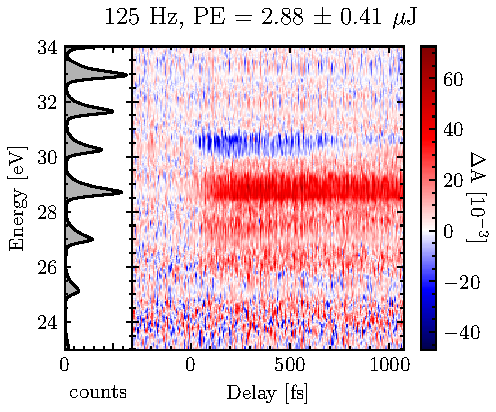
\includegraphics[width=0.4\textwidth]{figures/chap4/Delay123456_1430nm_125Hz_2p88uJ.pdf}
		\label{fig:125Hz_1430nm_Ge_ATAS:delay123456}}
	\qquad
	\subfloat[250 Hz ($M=2$)]{
		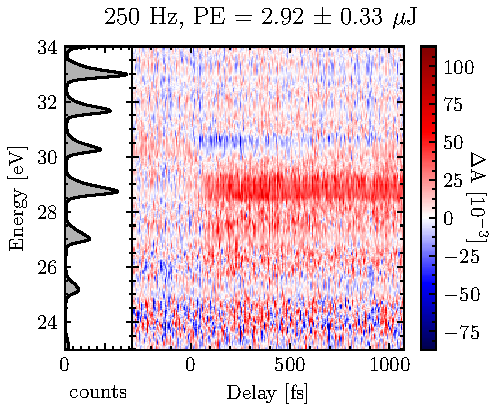
\includegraphics[width=0.4\textwidth]{figures/chap4/Delay89_1430nm_250Hz_2p92uJ.pdf}
		\label{fig:250Hz_1430nm_Ge_ATAS:delay89}}
	
	\caption{125 vs. 250 Hz measurements at $\lambda$ = 1430 nm. }
	\label{fig:125vs250Hz_1430nm_Ge_ATAS:delay}
	% datasets:
	% 125 Hz: \testdata\2019_08_15\125Hz\Delay1-6 averaged
	% 250 Hz: \testdata\2019_08_15\250Hz\Delay8,9 averaged
	% python script: \Python Scripts\Spectrometer\test\2019_08_15.py
\end{figure}

The fundamental wavelength was decreased by 20 nm to 1430 nm, where the absorption length in Ge is about 5\% shorter. For a fixed pulse energy, this increases the excitation fraction and thus the strength of the $\Delta A$ signal. Changing the wavelength also changes which initial and final states near the Fermi level are populated, according to the band structure calculations in \cref{fig:Ge_band_diagram}. Using this shorter wavelength we can observe a more robust sample response, as shown in \cref{fig:125vs250Hz_1430nm_Ge_ATAS:delay}.

At 1430 nm, we can see a sample response from 25.7 to 31 eV. From 25.7 to 30 eV, there is a broad increase in absorption, with the largest increase occuring between 28.4 and 29.5 eV. A decrease in absorption occurs between 30 and 31 eV. These features are present in both the 125 and 250 Hz data. The 30 eV negative delay feature persists in the 250 Hz dataset, but at $12 \times 10^{-3}$ it does not overwhelm the rest of the sample response. Further measurements were performed at either 125 Hz to suppress the static feature, or at 250 Hz to minimize data collection time.


\subsection{optimized ATAS Ge experimental results}

\subsection{post-experiment analysis: verify we didn't permanently damage sample}

\section{Data Analysis}

\subsection{description of data pipeline}
\subsubsection{going from 2D image to 1D spectra}

\begin{figure}
	\centering
	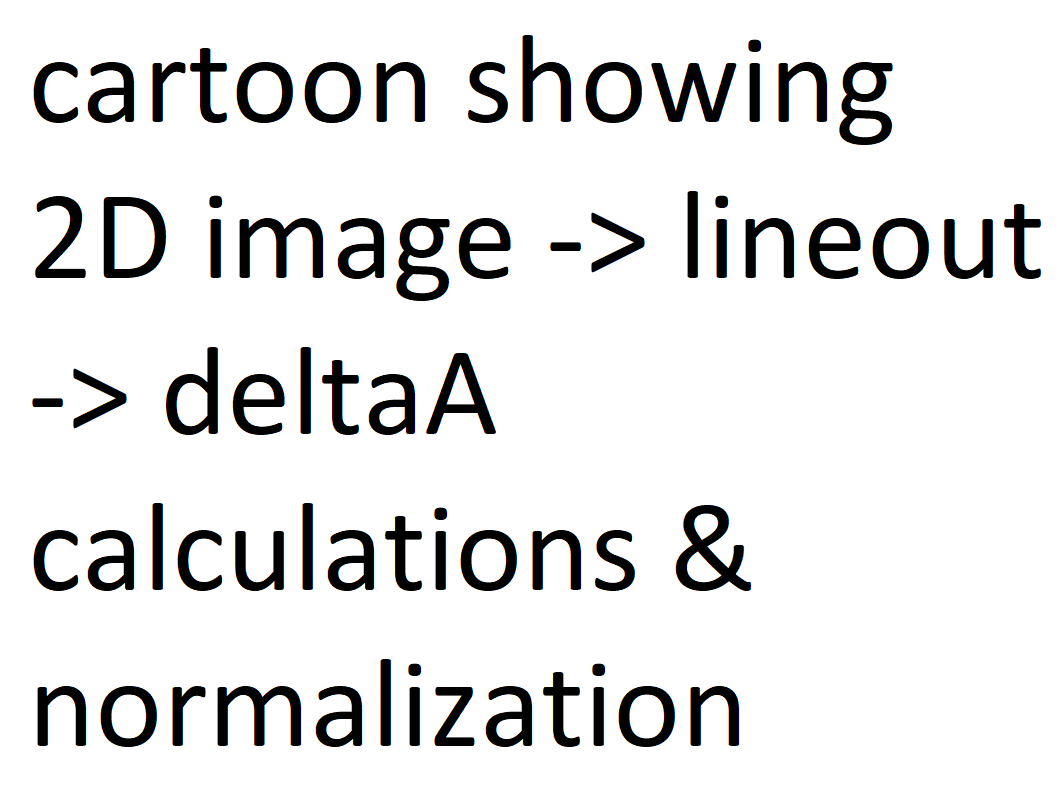
\includegraphics[width=0.75\textwidth]{figures/chap4/data_pipeline.png}
	\caption{this cartoon shows the data pipeline. it is an overview of all the processing steps i do on the data.}
	\label{fig:data_pipeline}
	% dataset: ???
	% python file: ???
\end{figure}

background subtraction, selecting a divergence window, normalization by exposure time \& divergence window, integration over divergence window
\subsubsection{energy calibration}

\begin{figure}
	\centering
	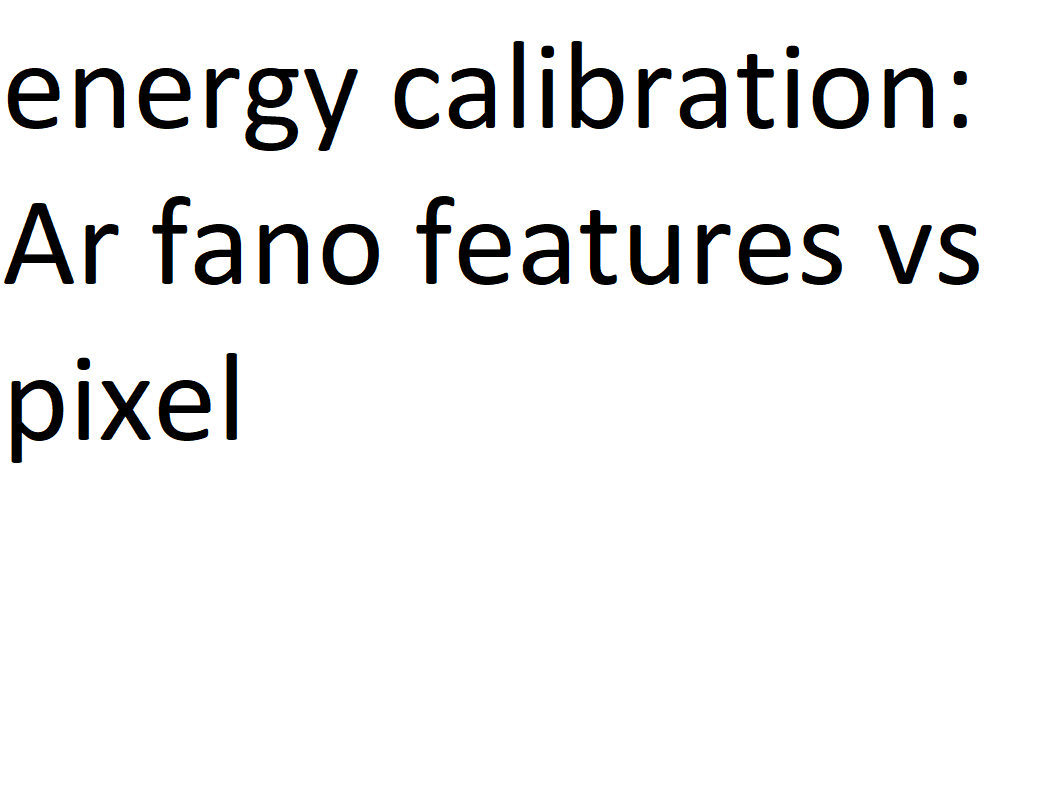
\includegraphics[width=0.75\textwidth]{figures/chap4/Ar_fano_cal.png}
	\caption{this figure shows the argon fano features vs pixel for the purpose of calibrating the spectrometer.}
	\label{fig:Ar_fano_calibration}
	% dataset: ???
	% python file: ???
\end{figure}



\subsubsection{$A$, $\Delta A$ calculation}

\subsection{systematic noise sources in our experiment}

\subsection{methods to numerically correct for harmonic noise and drift}

\subsection{frequency filtering to remove $\omega, 2 \omega$ oscillations}

\section{Physical Interpretation of spectra}
\subsection{decomposition of spectral response}
\subsection{description of observed dynamics}